%\newpage
%\subsection{Dataset}

Next, we apply our method to brain imaging data from the anonymized multimodal
neuroimaging ``Mother Of all Unification Studies'' (MOUS) dataset
\citep{schoffelen2019204}. The dataset contains functional Magnetic Resonance
Imaging (fMRI) and magneto-encephalography (MEG)
recordings of each 102 healthy Dutch adults who performed a reading
task in the scanner. Thirteen subjects were excluded from the analysis (12 MEG and 1 fMRI)
because of technical difficulties reading the files.
%
Subjects were exposed to a rapid serial visual presentation of Dutch words. The
word lists consisted of 120 sentences, and scrambled lists of the same words.
Each word was presented on the computer screen for 351ms on average (min: 300ms,
max: 1400ms). Successive words were separated by a blank screen for 300ms, and
successive sentences were separated by an empty screen for a few (3-4) seconds.

\subsubsection{fMRI preprocessing}
Results included in this manuscript come from preprocessing performed
using \emph{fMRIPrep} 20.0.7 (\citep{fmriprep1}; \citep{fmriprep2};
RRID:SCR\_016216), which is based on \emph{Nipype} 1.4.2
(\citep{nipype1}; \citep{nipype2}; RRID:SCR\_002502).

\begin{description}
\item[Anatomical data preprocessing]
A total of two T1-weighted (T1w) images per subject were found within the input BIDS
dataset. All of them were corrected for intensity non-uniformity (INU)
with \texttt{N4BiasFieldCorrection} \citep{n4}, distributed with ANTs
2.2.0 \citep[RRID:SCR\_004757]{ants}. The T1w-reference was then
skull-stripped with a \emph{Nipype} implementation of the
\texttt{antsBrainExtraction.sh} workflow (from ANTs), using OASIS30ANTs
as target template. Brain tissue segmentation of cerebrospinal fluid
(CSF), white-matter (WM) and gray-matter (GM) was performed on the
brain-extracted T1w using \texttt{fast} \citep[FSL 5.0.9,
RRID:SCR\_002823,][]{fsl_fast}. A T1w-reference map was computed after
registration of 2 T1w images (after INU-correction) using
\texttt{mri\_robust\_template} \citep[FreeSurfer 6.0.1,][]{fs_template}.
Brain surfaces were reconstructed using \texttt{recon-all}
\citep[FreeSurfer 6.0.1, RRID:SCR\_001847,][]{fs_reconall}, and the
brain mask estimated previously was refined with a custom variation of
the method to reconcile ANTs-derived and FreeSurfer-derived
segmentations of the cortical gray-matter of Mindboggle
\citep[RRID:SCR\_002438,][]{mindboggle}. Volume-based spatial
normalization to two standard spaces (MNI152NLin2009cAsym,
MNI152NLin6Asym) was performed through nonlinear registration with
\texttt{antsRegistration} (ANTs 2.2.0), using brain-extracted versions
of both T1w reference and the T1w template. The following templates were
selected for spatial normalization: \emph{ICBM 152 Nonlinear
Asymmetrical template version 2009c} {[}\citep{mni152nlin2009casym},
RRID:SCR\_008796; TemplateFlow ID: MNI152NLin2009cAsym{]}, \emph{FSL's
MNI ICBM 152 non-linear 6th Generation Asymmetric Average Brain
Stereotaxic Registration Model} {[}\citep{mni152nlin6asym},
RRID:SCR\_002823; TemplateFlow ID: MNI152NLin6Asym{]},
\item[Functional data preprocessing]
For each of the 2 BOLD runs found per subject, the following preprocessing was performed. First, a reference
volume and its skull-stripped version were generated using a custom
methodology of \emph{fMRIPrep}. Susceptibility distortion correction
(SDC) was omitted. The BOLD reference was then co-registered to the T1w
reference using \texttt{bbregister} (FreeSurfer) which implements
boundary-based registration \citep{bbr}. Co-registration was configured
with six degrees of freedom. Head-motion parameters with respect to the
BOLD reference (transformation matrices, and six corresponding rotation
and translation parameters) are estimated before any spatiotemporal
filtering using \texttt{mcflirt} \citep[FSL 5.0.9,][]{mcflirt}. BOLD
runs were slice-time corrected using \texttt{3dTshift} from AFNI
20160207 \citep[RRID:SCR\_005927]{afni}. The BOLD time-series were
resampled onto the following surfaces (FreeSurfer reconstruction
nomenclature): \emph{fsnative}, \emph{fsaverage5}. The BOLD time-series
(including slice-timing correction when applied) were resampled onto
their original, native space by applying the transforms to correct for
head-motion. These resampled BOLD time-series will be referred to as
\emph{preprocessed BOLD in original space}, or just \emph{preprocessed
BOLD}. The BOLD time-series were resampled into standard space,
generating a \emph{preprocessed BOLD run in MNI152NLin2009cAsym space}.
First, a reference volume and its skull-stripped version were generated
using a custom methodology of \emph{fMRIPrep}. Automatic removal of
motion artifacts using independent component analysis
\citep[ICA-AROMA,][]{aroma} was performed on the \emph{preprocessed BOLD
on MNI space} time-series after removal of non-steady state volumes and
spatial smoothing with an isotropic, Gaussian kernel of 6mm FWHM
(full-width half-maximum). Corresponding ``non-aggresively'' denoised
runs were produced after such smoothing.
% Additionally, the
% ``aggressive'' noise-regressors were collected and placed in the
% corresponding confounds file.
% Several confounding time-series were
% calculated based on the \emph{preprocessed BOLD}: framewise displacement
% (FD), DVARS and three region-wise global signals. FD and DVARS are
% calculated for each functional run, both using their implementations in
% \emph{Nipype} \citep[following the definitions by][]{power_fd_dvars}.
% The three global signals are extracted within the CSF, the WM, and the
% whole-brain masks. Additionally, a set of physiological regressors were
% extracted to allow for component-based noise correction
% \citep[\emph{CompCor},][]{compcor}. Principal components are estimated
% after high-pass filtering the \emph{preprocessed BOLD} time-series
% (using a discrete cosine filter with 128s cut-off) for the two
% \emph{CompCor} variants: temporal (tCompCor) and anatomical (aCompCor).
% tCompCor components are then calculated from the top 5\% variable voxels
% within a mask covering the subcortical regions. This subcortical mask is
% obtained by heavily eroding the brain mask, which ensures it does not
% include cortical GM regions. For aCompCor, components are calculated
% within the intersection of the aforementioned mask and the union of CSF
% and WM masks calculated in T1w space, after their projection to the
% native space of each functional run (using the inverse BOLD-to-T1w
% transformation). Components are also calculated separately within the WM
% and CSF masks. For each CompCor decomposition, the \emph{k} components
% with the largest singular values are retained, such that the retained
% components' time series are sufficient to explain 50 percent of variance
% across the nuisance mask (CSF, WM, combined, or temporal). The remaining
% components are dropped from consideration. The head-motion estimates
% calculated in the correction step were also placed within the
% corresponding confounds file. The confound time series derived from head
% motion estimates and global signals were expanded with the inclusion of
% temporal derivatives and quadratic terms for each
% \citep{confounds_satterthwaite_2013}. Frames that exceeded a threshold
% of 0.5 mm FD or 1.5 standardised DVARS were annotated as motion
% outliers.
% All resamplings can be performed with \emph{a single
% interpolation step} by composing all the pertinent transformations
% (i.e.~head-motion transform matrices, susceptibility distortion
% correction when available, and co-registrations to anatomical and output
% spaces). Gridded (volumetric) resamplings were performed using
% \texttt{antsApplyTransforms} (ANTs), configured with Lanczos
% interpolation to minimize the smoothing effects of other kernels
% \citep{lanczos}. Non-gridded (surface) resamplings were performed using
% \texttt{mri\_vol2surf} (FreeSurfer).
\end{description}

Many internal operations of \emph{fMRIPrep} use \emph{Nilearn} 0.6.2
\citep[RRID:SCR\_001362]{nilearn}, mostly within the functional
processing workflow. For more details of the pipeline, see
\href{https://fmriprep.readthedocs.io/en/latest/workflows.html}{the
section corresponding to workflows in \emph{fMRIPrep}'s documentation}.

% The above boilerplate text was automatically generated by fMRIPrep with
% the express intention that users should copy and paste this text into
% their manuscripts \emph{unchanged}. It is released under the
% \href{https://creativecommons.org/publicdomain/zero/1.0/}{CC0} license.

The preprocessed volumetric fMRI data was linearly projected to its closest surface
using nilearn \texttt{vol\_to\_surf} function with a 3 mm radius. A surface searchlight
analysis was then implemented by concatenating the surface
fMRI data within a 8mm radius of each vertex. For each subject and vertex, we
thus build an observation matrix $Y \in \mathbb{R}^{n \times d_y}$ of $n\approx$ 1400 words
by $d_y\approx40$ vertices per searchlight sphere. Each
of the columns of $Y$ is normalized to have zero mean and unit variance.

These multidimensional brain observations were to be accounted for (or decoded by) four features.

\subsubsection{Feature definition}

We aim to identify the word features that cause a variation in brain responses. We consider four distinct but collinear features.
%
First, 'Word Length' refers to the total number of letters. Word Length is expected to primarily cause a variation in the early evoked MEG responses (i.e. from 100 ms after stimulus onset) elicited by the retinotopically-tuned visual cortices (e.g. \citep{pegado2014timing}.).
%
Second, 'Word Frequency' indexes how frequently each word appears in Dutch and
was derived with the the Zipf logarithmic scale of \citep{van2014subtlex}
provided by the WordFreq package \citep{speerwordfreq}. Word Frequency is
expected to primarily cause a variation in the late evoked MEG responses (i.e.
from 400 ms) in the left frontal, temporal and parietal cortices
cortices \citep{kutas2011thirty,mccandliss2003visual}.
%
Third, 'Word Function' indicates whether each word is a content word (i.e. a
noun, a verb, an adjective or an adverb) or a function word (i.e. a preposition,
a conjunction, a determinant, a pronoun or a numeral), and was derived from
Spacy's part of speech tagger \citep{spacy2}. To our knowledge, this feature has
not been thoroughly investigated with fMRI and MEG. While its causal contribution to
reading processes in the brain thus remains unclear, this lexical feature can
nonetheless be expected to present similar brain patterns to word frequency.
%
Finally, to verify that B2B and other methods would not inadequately identify non-causal features, we added a dummy feature, constructed from a noisy combination of Word Length and Word Frequency:
$dummy = z(length) + z(frequency) + \mathcal{N}$, where $z$ normalizes features
and $\mathcal{N}$ is a random vector sampling Gaussian distribution (all terms
thus have a zero-mean and a unit-variance).

To account for the delay of blood oxygenation level dependent responses, the
features were convolved using the Glover hemodynamic response function
of nilearn's \texttt{compute\_regressor} function an oversampling of 16 and default parameters \citep{nilearn}.

This procedure yields an $X \in \mathbb{R}^{n \times d_x}$ matrix of $n\approx$
840 TR (Repetition Time: 2 sec.) by
$d_x=4$ features for each subject. Each of the columns of $X$ is normalized to
have a zero-mean and a unit variance.


\subsubsection{Models and statistics}

We compare B2B to four standard methods: Forward regression, Backward
regression, Regularized CCA and PLS, as implemented in scikit-learn
\citep{sklearn} and pyrcca \citep{bilenko2016pyrcca}, and optimized with nested cross-validation over twenty $l2$
regularization parameters logarithmically spaced between $10^{-4}$ and $10^4$
(for regression methods) or 1 to 4 canonical components (for cross-decomposition
methods).

We used the feature importance described in Algorithm \ref{algorithm:b2b_fi} to assess the extent to which each feature $X_i$ specifically improves the prediction of held-out $Y$ data, using a 5-fold cross-validation (with shuffled trials to homogeneize the distributions between the training and testing splits).

Each model was implemented for each subject and each time sample independently. Pairwise comparison between models were performed using a two-sided Wilcoxon test across subjects (n=90) using the average $\Delta R$ across time. Corresponding effect sizes are shown in Figure~\ref{fig:meg_results}, and p-values are reported below.


\begin{figure}
  \begin{center}
          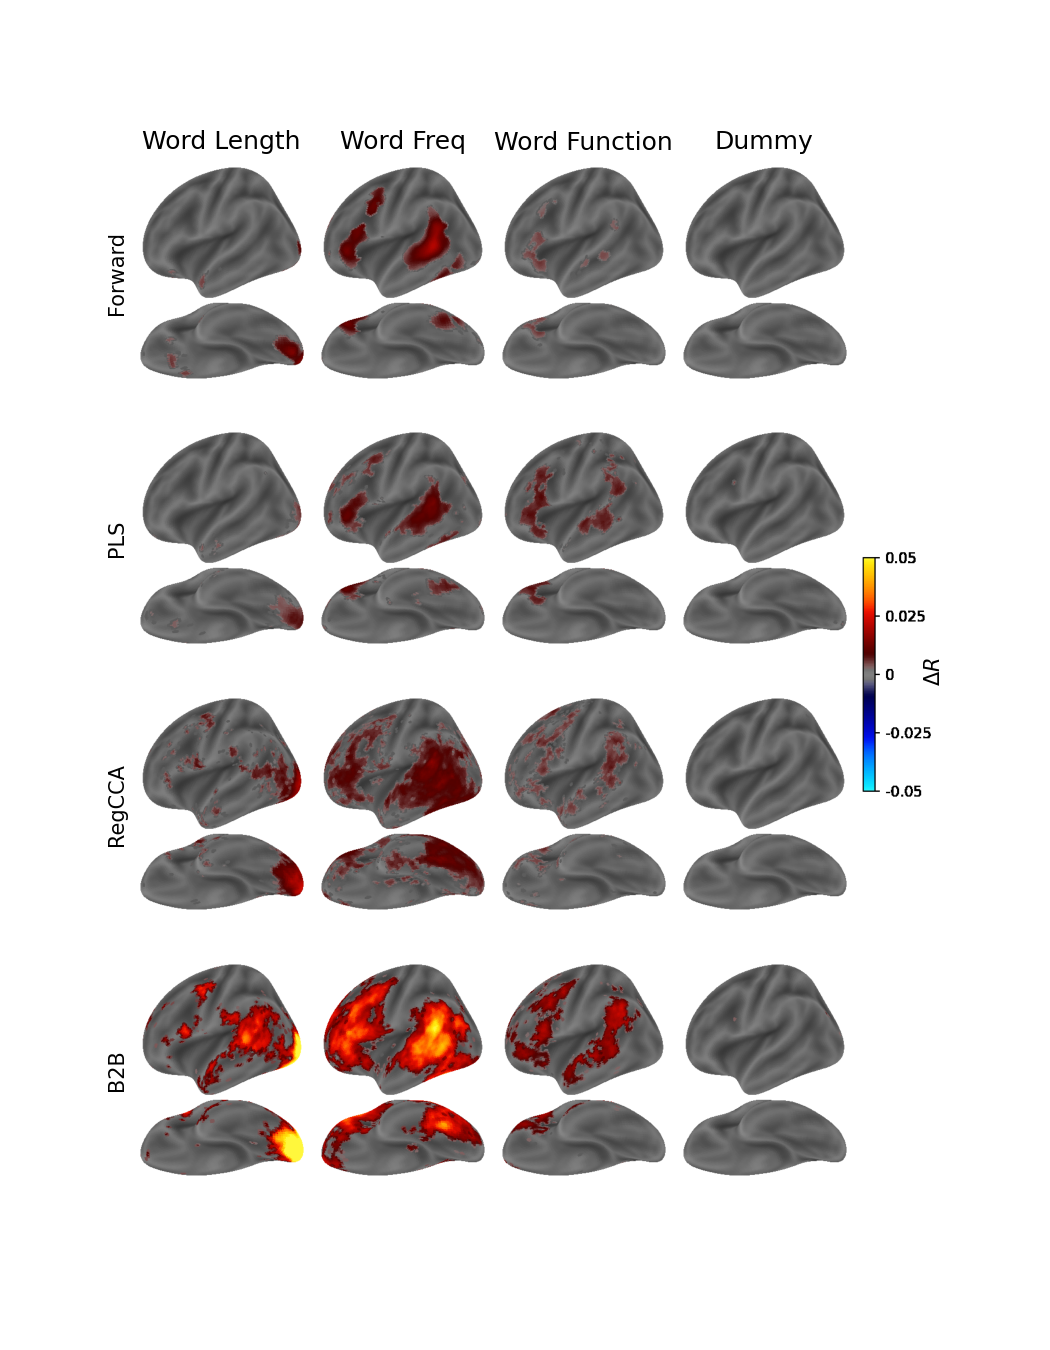
\includegraphics[width=.8\textwidth,
                       trim=1cm 1cm 1cm 2cm,
                       clip=True]{figures/fmri_delta_r.png}
          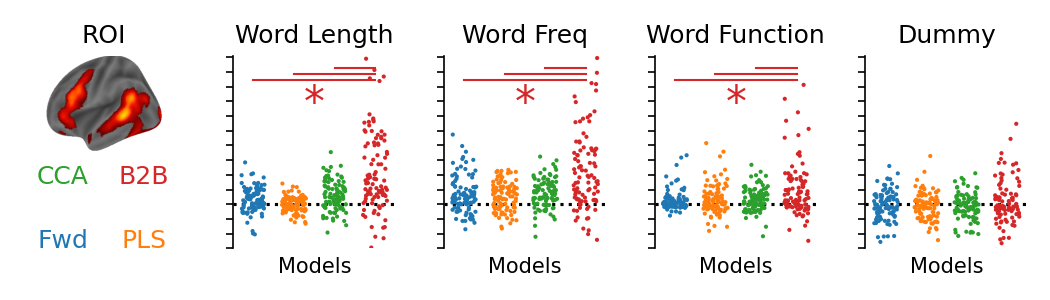
\includegraphics[width=.8\textwidth,
                       trim=0cm 0cm 0cm 0cm,
                       clip=True]{figures/fmri_strip.png}

      \label{fig:fmri_delta_r}
  \end{center}
  \caption{Top. Multiple models (rows) are compared on their ability to
  reliably predict out-of-sample fMRI signals evoked by words by quantifying
  the improvement of correlation coefficient $\Delta R$ for each of the four
  features (columns). Each cell displays the left hemisphere view laterally
  (top) or ventrally (bottom). Bottom left. Region
  of Interest (ROI), defined by the cortex vertices that were reliably
  predicted for by the gold standard Forward Model using all features and
  thresholded with a Wilcoxon at $p<0.001$ (uncorrected) across subjects. Bottom
  Right. Average $\Delta R$ within the ROI for each subject
  (dot); top horizontal lines indicate when B2B significantly outperforms
  other methods across subjects.}
\end{figure}


\subsubsection{fMRI Results}
We compared the ability of Forward regression, Backward regression, CCA, PLS
and B2B to estimate the causal contribution of four distinct but collinear
features on brain responses to words.

Supplementary Figure \ref{fig:fmri_supp} shows that the Backward model decodes
the dummy variable well above chance level. In addition, it decodes both Word
Length and Word Frequency across large sections of the cortex, even though
these features are known to primarily influence early visual cortex and
associative cortices respectively. These results illustrate that while Backward
modeling achieve high sensitivity, it is not valid to estimate the specific
causal contribution of collinear features.

On the contrary, the $\beta$
coefficients of the Forward model reveals the expected spatial specificity of
Word Length and Word Frequency, peaking the visual and temporal cortices
respectively. However such Forward coefficients may be variable across
subjects, and could thus underestimate the significance of each factor at each
vertex, as evaluated with a Wilcoxon tests across subjects. In principle, such
inter-subject variability could be less impactful with
multivariate observations methods such as CCA and PLS \citep{bilenko2016pyrcca,
king2018encoding}, but they fail to provide a single and interpretable coefficient
for each feature at each vertex.

In contrast, the $\hat S$ of an unbiased B2B (i.e. a B2B where $H$ is not
regularized) reaches higher levels of significance at each vertex
than the Forward $\beta$ \ref{fig:fmri_supp}. (Note that a direct
comparison between the Forward coefficients $\beta$ and those of B2B ($\hat S$)
is not feasible, as these two do not have the same units.)

To fairly compare the Forward, CCA, PLS and B2B methods on a common and robust
evaluation metric we compare them on their ability to improve $Y$
predictions of out-of-sample data when one factor is introduced into the model.
This analysis leads to a $\Delta R$ as described in Algorithm
\ref{algorithm:b2b_fi}). As expected, the Forward, CCA, PLS
and B2B method predicted that the Dummy Variable does not improve the $Y$
prediction. This confirms that these methods accurately rule out the known
non-causal factor.

The average $\Delta R$ across subjects is displayed for each model and each
feature in \ref{fig:fmri_delta_r}. Overall, B2B favorably compares to baseline models.
To quantify this assessment, we compare for each subject separately
the average $\Delta R$ across vertices obtained between B2B and each
baseline model. To limit the inclusion of uninformative brain regions in this
summary, we restrict the analysis to vertices which can be reliably accounted
for by the Forward model ($p<.001$, not corrected across vertices)
\ref{fig:fmri_delta_r}. The results show that B2B significantly outperforms all
baseline models on all factors (all $p<0.0001$) but the dummy variable
(min $p=0.0852$).
